\chapter{THIẾT KẾ PHẦN CỨNG VÀ TRUYỀN THÔNG IOT}
\label{ch:chuong2}

\section{Sơ đồ mạch mô phỏng Wokwi chuẩn hệ thống}
\label{sec:so_do_mach_wokwi}

Để bảo đảm tính đúng đắn về nguyên lý điện tử và hạn chế tối đa rủi ro chập cháy trước khi triển khai trên linh kiện thật, toàn bộ hệ thống phần cứng IoT của SmartDorm đã được thiết kế và kiểm thử thành công trên nền tảng mô phỏng nhúng trực tuyến Wokwi. 

Hình \ref{fig:so_do_wokwi} thể hiện sơ đồ mạch điện tử hoàn chỉnh được xuất trực tiếp từ dự án mô phỏng Wokwi của hệ thống.

\begin{figure}[H]
\centering
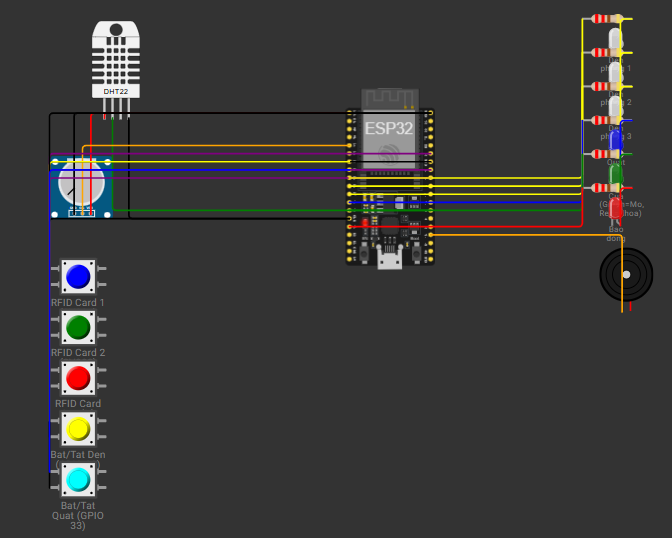
\includegraphics[width=0.95\textwidth]{figures/so_do_mach_mo_phong_wokwi.png}
\caption{Sơ đồ mạch mô phỏng hoàn chỉnh của nút mạng SmartDorm trên nền tảng Wokwi}
\label{fig:so_do_wokwi}
\end{figure}

Sơ đồ mạch mô phỏng trên Wokwi tích hợp đầy đủ các khối chức năng tương thích 100\% với thiết kế vật lý:
\begin{itemize}
    \item \textbf{Khối xử lý trung tâm:} Sử dụng vi điều khiển ESP32 DevKit V1 (30 chân) đóng vai trò điều phối toàn bộ tín hiệu cảm biến, thuật toán xử lý ngắt và giao thức truyền thông không dây Wi-Fi.
    \item \textbf{Khối cảm biến môi trường:} Cảm biến DHT22 được cấp nguồn 3.3V và gửi dữ liệu số về chân GPIO 4; Cảm biến khí gas/khói MQ-2 được cấp nguồn 5V gửi tín hiệu điện áp về chân GPIO 34.
    \item \textbf{Khối điều khiển chấp hành:} Module relay 4 kênh nhận tín hiệu kích hoạt mức logic từ các chân GPIO 25, 26, 14, 12 để điều khiển đèn chiếu sáng, quạt thông gió và chốt khóa cửa điện từ Solenoid.
    \item \textbf{Khối cảnh báo âm thanh và thị giác:} Còi Active Buzzer kết nối với chân GPIO 15 và đèn LED đỏ cảnh báo PCCC kết nối với chân GPIO 13.
    \item \textbf{Khối nút nhấn tương tác và mô phỏng an ninh:} 5 nút nhấn nhả (Tactile Buttons) được kết nối với các chân GPIO 32 (Đèn), GPIO 33 (Quạt), GPIO 18 (Thẻ SV001 hợp lệ), GPIO 19 (Thẻ SV002 hợp lệ) và GPIO 21 (Thẻ Lạ không hợp lệ).
\end{itemize}

\section{Bảng phân bổ chân GPIO ESP32}
\label{sec:bang_phan_bo_gpio}

Vi điều khiển ESP32 NodeMCU-32S có 30 chân cắm được bố trí thành hai hàng chân hai bên bo mạch. Để bảo đảm hệ thống hoạt động ổn định, tránh xung đột các chân strapping (chân nạp bootloader), bảng phân bổ chân GPIO được quy hoạch nghiêm ngặt như trong Bảng \ref{tab:phan_bo_gpio}.

\begin{table}[H]
\centering
\small
\begin{tabularx}{\textwidth}{|c|p{2.2cm}|p{2.5cm}|p{2.0cm}|X|}
\hline
\textbf{STT} & \textbf{Chân ESP32} & \textbf{Thiết bị ngoại vi} & \textbf{Chế độ chân} & \textbf{Chức năng trong hệ thống} \\
\hline
1 & \textbf{VIN (5V)} & Nguồn chung 5V & Power Out & Cấp nguồn 5V cho cảm biến MQ-2 và Bo Relay 4 kênh \\
\hline
2 & \textbf{3V3 (3.3V)} & Nguồn DHT22 & Power Out & Cấp nguồn 3.3V DC độc lập cho cảm biến vi khí hậu DHT22 \\
\hline
3 & \textbf{GND} & Mass chung (0V) & Ground & Nối mass chung cho toàn bộ cảm biến, nút bấm, relay và buzzer \\
\hline
4 & \textbf{GPIO 34} & Cảm biến Gas MQ-2 & INPUT & Đọc tín hiệu nồng độ khí gas / khói (chân Analog/Digital) \\
\hline
5 & \textbf{GPIO 4} & Cảm biến DHT22 & INPUT & Nhận chuỗi xung dữ liệu số đo nhiệt độ ($^\circ\text{C}$) và độ ẩm (\%) \\
\hline
6 & \textbf{GPIO 32} & Nút bấm Đèn & PULLUP & Nút bấm vật lý bật/tắt Đèn phòng (chống dội phím phần mềm) \\
\hline
7 & \textbf{GPIO 33} & Nút bấm Quạt & PULLUP & Nút bấm vật lý bật/tắt Quạt thông gió \\
\hline
8 & \textbf{GPIO 18} & Thẻ SV001 (An) & PULLUP & Mô phỏng quẹt thẻ RFID hợp lệ: mở cửa 4s, còi bíp 1 tiếng \\
\hline
9 & \textbf{GPIO 19} & Thẻ SV002 (Bình) & PULLUP & Mô phỏng quẹt thẻ RFID hợp lệ của bạn cùng phòng \\
\hline
10 & \textbf{GPIO 21} & Thẻ Lạ (Vi phạm) & PULLUP & Mô phỏng quẹt thẻ không có quyền: còi kêu 3 tiếng, khóa giữ đóng \\
\hline
11 & \textbf{GPIO 25} & Relay 1 (Đèn 1) & OUTPUT & Điều khiển đóng/ngắt nguồn điện cho bóng đèn chiếu sáng 1 \\
\hline
12 & \textbf{GPIO 26} & Relay 2 (Đèn 2) & OUTPUT & Điều khiển đóng/ngắt nguồn điện cho bóng đèn chiếu sáng 2 \\
\hline
13 & \textbf{GPIO 14} & Relay 3 (Quạt) & OUTPUT & Kích hoạt quạt thông gió (tự bật khi gas $\ge 80\%$ để hút khí) \\
\hline
14 & \textbf{GPIO 12} & Relay 4 (Khóa) & OUTPUT & Kích hoạt đóng/mở chốt khóa cửa điện từ Solenoid \\
\hline
15 & \textbf{GPIO 15} & Còi Active Buzzer & OUTPUT & Phát âm thanh bíp cảnh báo an ninh hoặc còi hú khẩn cấp PCCC \\
\hline
16 & \textbf{GPIO 13} & LED Đỏ Cảnh Báo & OUTPUT & Đèn chớp cảnh báo thị giác khi nồng độ gas vượt ngưỡng an toàn \\
\hline
\end{tabularx}
\caption{Bảng phân bổ chi tiết các chân GPIO trên vi điều khiển ESP32 NodeMCU-32S}
\label{tab:phan_bo_gpio}
\end{table}

\section{Thuyết minh kỹ thuật lắp ráp bo mạch phần cứng thực tế}
\label{sec:thuyet_minh_lap_rap}

Quy trình đấu nối và lắp ráp phần cứng thực tế được xây dựng chi tiết theo tài liệu hướng dẫn kỹ thuật của dự án, tối ưu hóa theo phương án cắm dây Cái – Đực kết hợp bo cắm lỗ Breadboard MB-102 nhằm bảo đảm mạch điện gọn gàng, cách điện an toàn và thuận tiện cho việc kiểm tra.

\subsection{Thiết lập 2 thanh nguồn chung trên Breadboard}
Trên bo cắm thử nghiệm Breadboard MB-102, hai dải lỗ chạy dọc ở mép ngoài cùng được sử dụng để phân phối nguồn điện:
\begin{itemize}
    \item \textbf{Thanh nguồn 5V (Dải sọc Đỏ bên trái):} Nối bằng dây Cái - Đực màu Đỏ từ chân \texttt{VIN} (chân số 15 bên trái ESP32) sang thanh nguồn. Dải này duy trì điện áp 5V nuôi cảm biến khí gas MQ-2 và module relay 4 kênh.
    \item \textbf{Thanh Mass chung 0V GND (Dải sọc Xanh bên trái):} Nối bằng dây Cái - Đực màu Đen từ chân \texttt{GND} (chân số 14 bên trái ESP32) sang thanh mass. Toàn bộ các cực âm của linh kiện đều được đấu chung vào dải này để bảo đảm đẳng thế 0V.
    \item \textbf{Cấp nguồn riêng 3.3V cho DHT22:} Để tránh quá tải nguồn và loại bỏ xung nhiễu từ các cuộn hút relay, chân cấp nguồn \texttt{+} của cảm biến DHT22 được cắm trực tiếp vào chân \texttt{3V3} (chân số 16 bên phải ESP32).
\end{itemize}

\subsection{Quy tắc cắm nút nhấn 4 chân chéo góc chống chập mạch}
Để khắc phục hoàn toàn lỗi nút bấm bị dính tiếp điểm thường gặp, cả 5 nút bấm được cắm vắt ngang qua rãnh lõm cách điện ở giữa Breadboard:
\begin{itemize}
    \item \textbf{Chân 1 (Góc trên bên trái):} Cắm dây về chân GPIO tương ứng trên ESP32 (GPIO 32, 33, 18, 19, 21). Vi điều khiển được cấu hình kích hoạt điện trở kéo lên nội (\texttt{INPUT\_PULLUP}), duy trì mức điện áp 3.3V khi nút không bấm.
    \item \textbf{Chân 4 (Góc dưới bên phải):} Cắm dây nối thẳng về Thanh Mass Chung (\texttt{GND}). Khi người dùng nhấn nút, tiếp điểm đóng lại kéo điện áp chân GPIO xuống 0V (mức LOW).
    \item Hai chân còn lại của nút bấm được để trống hoàn toàn. Nguyên lý đấu dây chéo góc bảo đảm mạch không bao giờ bị ngắn mạch nội tại.
\end{itemize}

\subsection{Đấu nối Module Rơ-le (Relay) 5V 4 kênh cách ly quang}
Module relay sử dụng optocoupler cách ly hoàn toàn giữa mạch điều khiển logic 3.3V của ESP32 và mạch đóng cắt phụ tải:
\begin{itemize}
    \item Chân \texttt{VCC} của bo relay nối vào Thanh Nguồn 5V chung; chân \texttt{GND} nối vào Thanh Mass chung.
    \item Các chân tín hiệu điều khiển \texttt{IN1, IN2, IN3, IN4} nối lần lượt vào các chân GPIO 25, 26, 14, 12 của ESP32.
    \item Module relay hoạt động theo mức kích hoạt tích cực thấp (Active LOW): Khi chân GPIO xuất mức 0V, rơ-le đóng tiếp điểm thường mở (NO - Normally Open), cấp điện cho thiết bị.
\end{itemize}

\subsection{Đấu nối Cảm biến DHT22 và MQ-2}
\begin{itemize}
    \item \textbf{Cảm biến DHT22:} Chân \texttt{+} nối chân 3V3 của ESP32; chân \texttt{-} nối Thanh Mass GND; chân tín hiệu số \texttt{out} nối chân GPIO 4.
    \item \textbf{Cảm biến MQ-2:} Chân \texttt{VCC} nối Thanh Nguồn 5V (dây đốt nhiệt cần nguồn 5V để nung nóng lớp nhạy khí $SnO_2$); chân \texttt{GND} nối Mass chung; chân tín hiệu điện áp tương tự nối chân GPIO 34.
\end{itemize}

\section{Khung định vị dành cho ảnh bo mạch thực tế sau lắp ráp}
\label{sec:khung_anh_thuc_te}

Để bảo đảm tính khoa học và trung thực của báo cáo, theo yêu cầu của tác giả, hệ thống không sử dụng bất kỳ hình ảnh nhân tạo hoặc ảnh đồ họa giả lập nào cho các linh kiện vật lý. Khu vực dưới đây được bố trí trang trọng làm khung định vị chuẩn để tác giả chèn hình ảnh bo mạch phần cứng thực tế sau khi hoàn thành lắp ráp và thử nghiệm nghiệm thu:

\begin{figure}[H]
\centering
\fcolorbox{blue!80!black}{gray!4}{%
  \begin{minipage}[c][8.5cm][c]{14.5cm}
    \centering
    \vspace{0.5cm}
    {\Huge \bfseries [ KHU VỰC ĐỊNH VỊ ẢNH BO MẠCH THỰC TẾ ]}\\[0.6cm]
    {\large \bfseries HỆ THỐNG PHẦN CỨNG IOT SMARTDORM HOÀN THIỆN}\\[0.3cm]
    {\normalsize (Bao gồm: Bo ESP32 CP2102 Type-C, Breadboard 5 nút bấm, Còi Buzzer 5V,}\\[0.1cm]
    {\normalsize Module Relay 4 kênh cách ly quang, Cảm biến vi khí hậu DHT22 và Cảm biến khí Gas MQ-2)}\\[1.0cm]
    {\itshape\small * Hình ảnh chụp thực tế của tác giả sẽ được cập nhật tại đây sau khi hoàn tất công tác nghiệm thu phần cứng *}
    \vspace{0.5cm}
  \end{minipage}%
}
\caption{Hình ảnh bo mạch phần cứng thực tế của nút mạng IoT SmartDorm sau khi lắp ráp hoàn thiện}
\label{fig:anh_bo_mach_thuc_te}
\end{figure}

\section{Thiết kế Firmware điều khiển trên vi điều khiển ESP32}
\label{sec:firmware_esp32}

Firmware của nút mạng IoT được phát triển bằng ngôn ngữ C++ trên nền tảng PlatformIO (Arduino Framework), tối ưu hóa tốc độ thực thi với kiến trúc hướng sự kiện không nghẽn (Non-blocking Architecture) sử dụng biến đếm thời gian thực \texttt{millis()}:

\begin{itemize}
    \item \textbf{Thuật toán chống dội phím (Debounce Algorithm):} Các nút bấm vật lý sinh ra các dao động điện áp tiếp điểm trong khoảng thời gian từ $10$ đến $30\text{ ms}$. Firmware kiểm tra trạng thái phím ổn định sau $50\text{ ms}$ trước khi xác nhận lệnh, loại bỏ hiện tượng kích hoạt lặp lệnh điều khiển.
    \item \textbf{Cơ chế chu kỳ lấy mẫu cảm biến không chặn:} Cảm biến DHT22 và MQ-2 được đọc định kỳ mỗi $3000\text{ ms}$ mà không sử dụng hàm \texttt{delay()}, bảo đảm luồng mạng MQTT luôn duy trì kết nối liên tục (Keep-Alive).
    \item \textbf{Cơ chế bảo vệ khẩn cấp tại chỗ (Local Fail-Safe Engine):} Đây là tính năng an toàn sống còn của hệ thống. Khi cảm biến MQ-2 đo được nồng độ gas đạt ngưỡng $\ge 80\%$, firmware ESP32 ngay lập tức thực thi logic phần cứng tại chỗ:
    \begin{enumerate}
        \item Kích hoạt chân GPIO 15 điều khiển còi hú liên tục không ngắt quãng.
        \item Ngắt toàn bộ relay điện phòng (chuyển chân GPIO 25, 26 sang mức HIGH) nhằm cắt nguồn điện đèn và thiết bị sinh hoạt, triệt tiêu nguy cơ phóng điện phát sinh tia lửa gây hỏa hoạn.
        \item Bật relay số 3 (GPIO 14) kích hoạt quạt thông gió hoạt động hết công suất để hút xả khí gas rò rỉ ra ngoài.
        \item Xuất bản bản tin MQTT khẩn cấp có độ ưu tiên cao nhất lên chủ đề cảnh báo.
    \end{enumerate}
    Toàn bộ quá trình bảo vệ khẩn cấp tại chỗ này diễn ra trong vòng dưới $100\text{ ms}$, hoàn toàn độc lập với việc có kết nối mạng Internet hay không!
\end{itemize}

Đoạn mã C++ cốt lõi xử lý an toàn tại chỗ trên ESP32 được thể hiện trong Listing \ref{lst:firmware_failsafe}:

\begin{lstlisting}[language=C++, caption={Thuật toán bảo vệ an toàn PCCC tại chỗ trên Firmware ESP32}, label={lst:firmware_failsafe}]
void checkSafetyAndSensors() {
  unsigned long currentMillis = millis();
  if (currentMillis - lastSensorRead >= 3000) {
    lastSensorRead = currentMillis;
    float temp = dht.readTemperature();
    float hum = dht.readHumidity();
    int gasRaw = analogRead(GAS_PIN);
    float gasPercent = (gasRaw / 4095.0) * 100.0;

    // KIEM TRA NGUONG PCCC NGUY HIEM (>= 80%)
    if (gasPercent >= 80.0) {
      // 1. Kich hoat coi bao dong tai cho
      digitalWrite(BUZZER_PIN, HIGH);
      digitalWrite(ALERT_LED_PIN, HIGH);
      // 2. NGAT TOAN BO NGUON DIEN PHONG (Relay Active LOW -> set HIGH de ngat)
      digitalWrite(RELAY_LIGHT1_PIN, HIGH);
      digitalWrite(RELAY_LIGHT2_PIN, HIGH);
      // 3. BAT QUAT THONG GIO GIAI PHONG KHI GAS (set LOW de bat)
      digitalWrite(RELAY_FAN_PIN, LOW);
      
      // 4. Phat ban tin MQTT khan cap
      publishEmergencyAlert("GAS_LEAK", "CRITICAL", gasPercent);
    }
  }
}
\end{lstlisting}

\section{Hạ tầng truyền thông mạng IoT}
\label{sec:truyen_thong_iot}

\subsection{Giao thức MQTT và quy hoạch Topic phân cấp}
Giao thức MQTT (Message Queuing Telemetry Transport) được lựa chọn làm giao thức truyền thông chính nhờ các đặc tính: gói tin nhẹ (header chỉ 2 bytes), hoạt động theo mô hình Publish/Subscribe tách biệt không gian, và hỗ trợ độ tin cậy tin nhắn mức QoS 1 (At least once delivery) có xác nhận gói tin PUBACK.

Hệ thống quy hoạch không gian Topic chuẩn phân cấp theo cấu trúc:
\begin{itemize}
    \item \texttt{dorm/\{building\}/\{floor\}/\{room\}/telemetry}: Bo ESP32 định kỳ xuất bản dữ liệu vi khí hậu và nồng độ khí gas.
    \item \texttt{dorm/\{building\}/\{floor\}/\{room\}/access}: Xuất bản sự kiện quẹt thẻ RFID (UID thẻ, kết quả xác thực).
    \item \texttt{dorm/\{building\}/\{floor\}/\{room\}/status}: Xuất bản phản hồi trạng thái thiết bị thực tế từ phần cứng về backend.
    \item \texttt{dorm/\{building\}/\{floor\}/\{room\}/command}: Backend xuất bản lệnh điều khiển thiết bị (Bật/Tắt, Mở cửa, Ngắt nguồn) xuống ESP32.
    \item \texttt{dorm/emergency/broadcast}: Kênh phát sóng sự cố khẩn cấp trên toàn ký túc xá.
\end{itemize}

\subsection{Giao thức WebSockets thời gian thực (Socket.IO)}
Trong khi MQTT phụ trách truyền thông giữa phần cứng nhúng và máy chủ backend, giao thức WebSockets (thông qua thư viện Socket.IO) đảm nhận vai trò kết nối liên tục toàn song công (Full-duplex) giữa máy chủ backend và trình duyệt web. 

Khi nhận được gói tin telemetry hoặc sự kiện an ninh từ MQTT, Backend lập tức phân phối thông tin đến đúng phòng ảo (\texttt{roomId room}) của các máy khách đang mở trình duyệt. Nhờ đó, độ trễ cập nhật giao diện web đạt mức dưới $15\text{ ms}$, mang lại trải nghiệm tương tác mượt mà và trực quan tức thì.

\newpage
